\documentclass[1p]{elsarticle_modified}
%\bibliographystyle{elsarticle-num}

%\usepackage[colorlinks]{hyperref}
%\usepackage{abbrmath_seonhwa} %\Abb, \Ascr, \Acal ,\Abf, \Afrak
\usepackage{amsfonts}
\usepackage{amssymb}
\usepackage{amsmath}
\usepackage{amsthm}
\usepackage{scalefnt}
\usepackage{amsbsy}
\usepackage{kotex}
\usepackage{caption}
\usepackage{subfig}
\usepackage{color}
\usepackage{graphicx}
\usepackage{xcolor} %% white, black, red, green, blue, cyan, magenta, yellow
\usepackage{float}
\usepackage{setspace}
\usepackage{hyperref}

\usepackage{tikz}
\usetikzlibrary{arrows}

\usepackage{multirow}
\usepackage{array} % fixed length table
\usepackage{hhline}

%%%%%%%%%%%%%%%%%%%%%
\makeatletter
\renewcommand*\env@matrix[1][\arraystretch]{%
	\edef\arraystretch{#1}%
	\hskip -\arraycolsep
	\let\@ifnextchar\new@ifnextchar
	\array{*\c@MaxMatrixCols c}}
\makeatother %https://tex.stackexchange.com/questions/14071/how-can-i-increase-the-line-spacing-in-a-matrix
%%%%%%%%%%%%%%%

\usepackage[normalem]{ulem}

\newcommand{\msout}[1]{\ifmmode\text{\sout{\ensuremath{#1}}}\else\sout{#1}\fi}
%SOURCE: \msout is \stkout macro in https://tex.stackexchange.com/questions/20609/strikeout-in-math-mode

\newcommand{\cancel}[1]{
	\ifmmode
	{\color{red}\msout{#1}}
	\else
	{\color{red}\sout{#1}}
	\fi
}

\newcommand{\add}[1]{
	{\color{blue}\uwave{#1}}
}

\newcommand{\replace}[2]{
	\ifmmode
	{\color{red}\msout{#1}}{\color{blue}\uwave{#2}}
	\else
	{\color{red}\sout{#1}}{\color{blue}\uwave{#2}}
	\fi
}

\newcommand{\Sol}{\mathcal{S}} %segment
\newcommand{\D}{D} %diagram
\newcommand{\A}{\mathcal{A}} %arc


%%%%%%%%%%%%%%%%%%%%%%%%%%%%%5 test

\def\sl{\operatorname{\textup{SL}}(2,\Cbb)}
\def\psl{\operatorname{\textup{PSL}}(2,\Cbb)}
\def\quan{\mkern 1mu \triangleright \mkern 1mu}

\theoremstyle{definition}
\newtheorem{thm}{Theorem}[section]
\newtheorem{prop}[thm]{Proposition}
\newtheorem{lem}[thm]{Lemma}
\newtheorem{ques}[thm]{Question}
\newtheorem{cor}[thm]{Corollary}
\newtheorem{defn}[thm]{Definition}
\newtheorem{exam}[thm]{Example}
\newtheorem{rmk}[thm]{Remark}
\newtheorem{alg}[thm]{Algorithm}

\newcommand{\I}{\sqrt{-1}}
\begin{document}

%\begin{frontmatter}
%
%\title{Boundary parabolic representations of knots up to 8 crossings}
%
%%% Group authors per affiliation:
%\author{Yunhi Cho} 
%\address{Department of Mathematics, University of Seoul, Seoul, Korea}
%\ead{yhcho@uos.ac.kr}
%
%
%\author{Seonhwa Kim} %\fnref{s_kim}}
%\address{Center for Geometry and Physics, Institute for Basic Science, Pohang, 37673, Korea}
%\ead{ryeona17@ibs.re.kr}
%
%\author{Hyuk Kim}
%\address{Department of Mathematical Sciences, Seoul National University, Seoul 08826, Korea}
%\ead{hyukkim@snu.ac.kr}
%
%\author{Seokbeom Yoon}
%\address{Department of Mathematical Sciences, Seoul National University, Seoul, 08826,  Korea}
%\ead{sbyoon15@snu.ac.kr}
%
%\begin{abstract}
%We find all boundary parabolic representation of knots up to 8 crossings.
%
%\end{abstract}
%\begin{keyword}
%    \MSC[2010] 57M25 
%\end{keyword}
%
%\end{frontmatter}

%\linenumbers
%\tableofcontents
%
\newcommand\colored[1]{\textcolor{white}{\rule[-0.35ex]{0.8em}{1.4ex}}\kern-0.8em\color{red} #1}%
%\newcommand\colored[1]{\textcolor{white}{ #1}\kern-2.17ex	\textcolor{white}{ #1}\kern-1.81ex	\textcolor{white}{ #1}\kern-2.15ex\color{red}#1	}

{\Large $\underline{12a_{0727}~(K12a_{0727})}$}

\setlength{\tabcolsep}{10pt}
\renewcommand{\arraystretch}{1.6}
\vspace{1cm}\begin{tabular}{m{100pt}>{\centering\arraybackslash}m{274pt}}
\multirow{5}{120pt}{
	\centering
	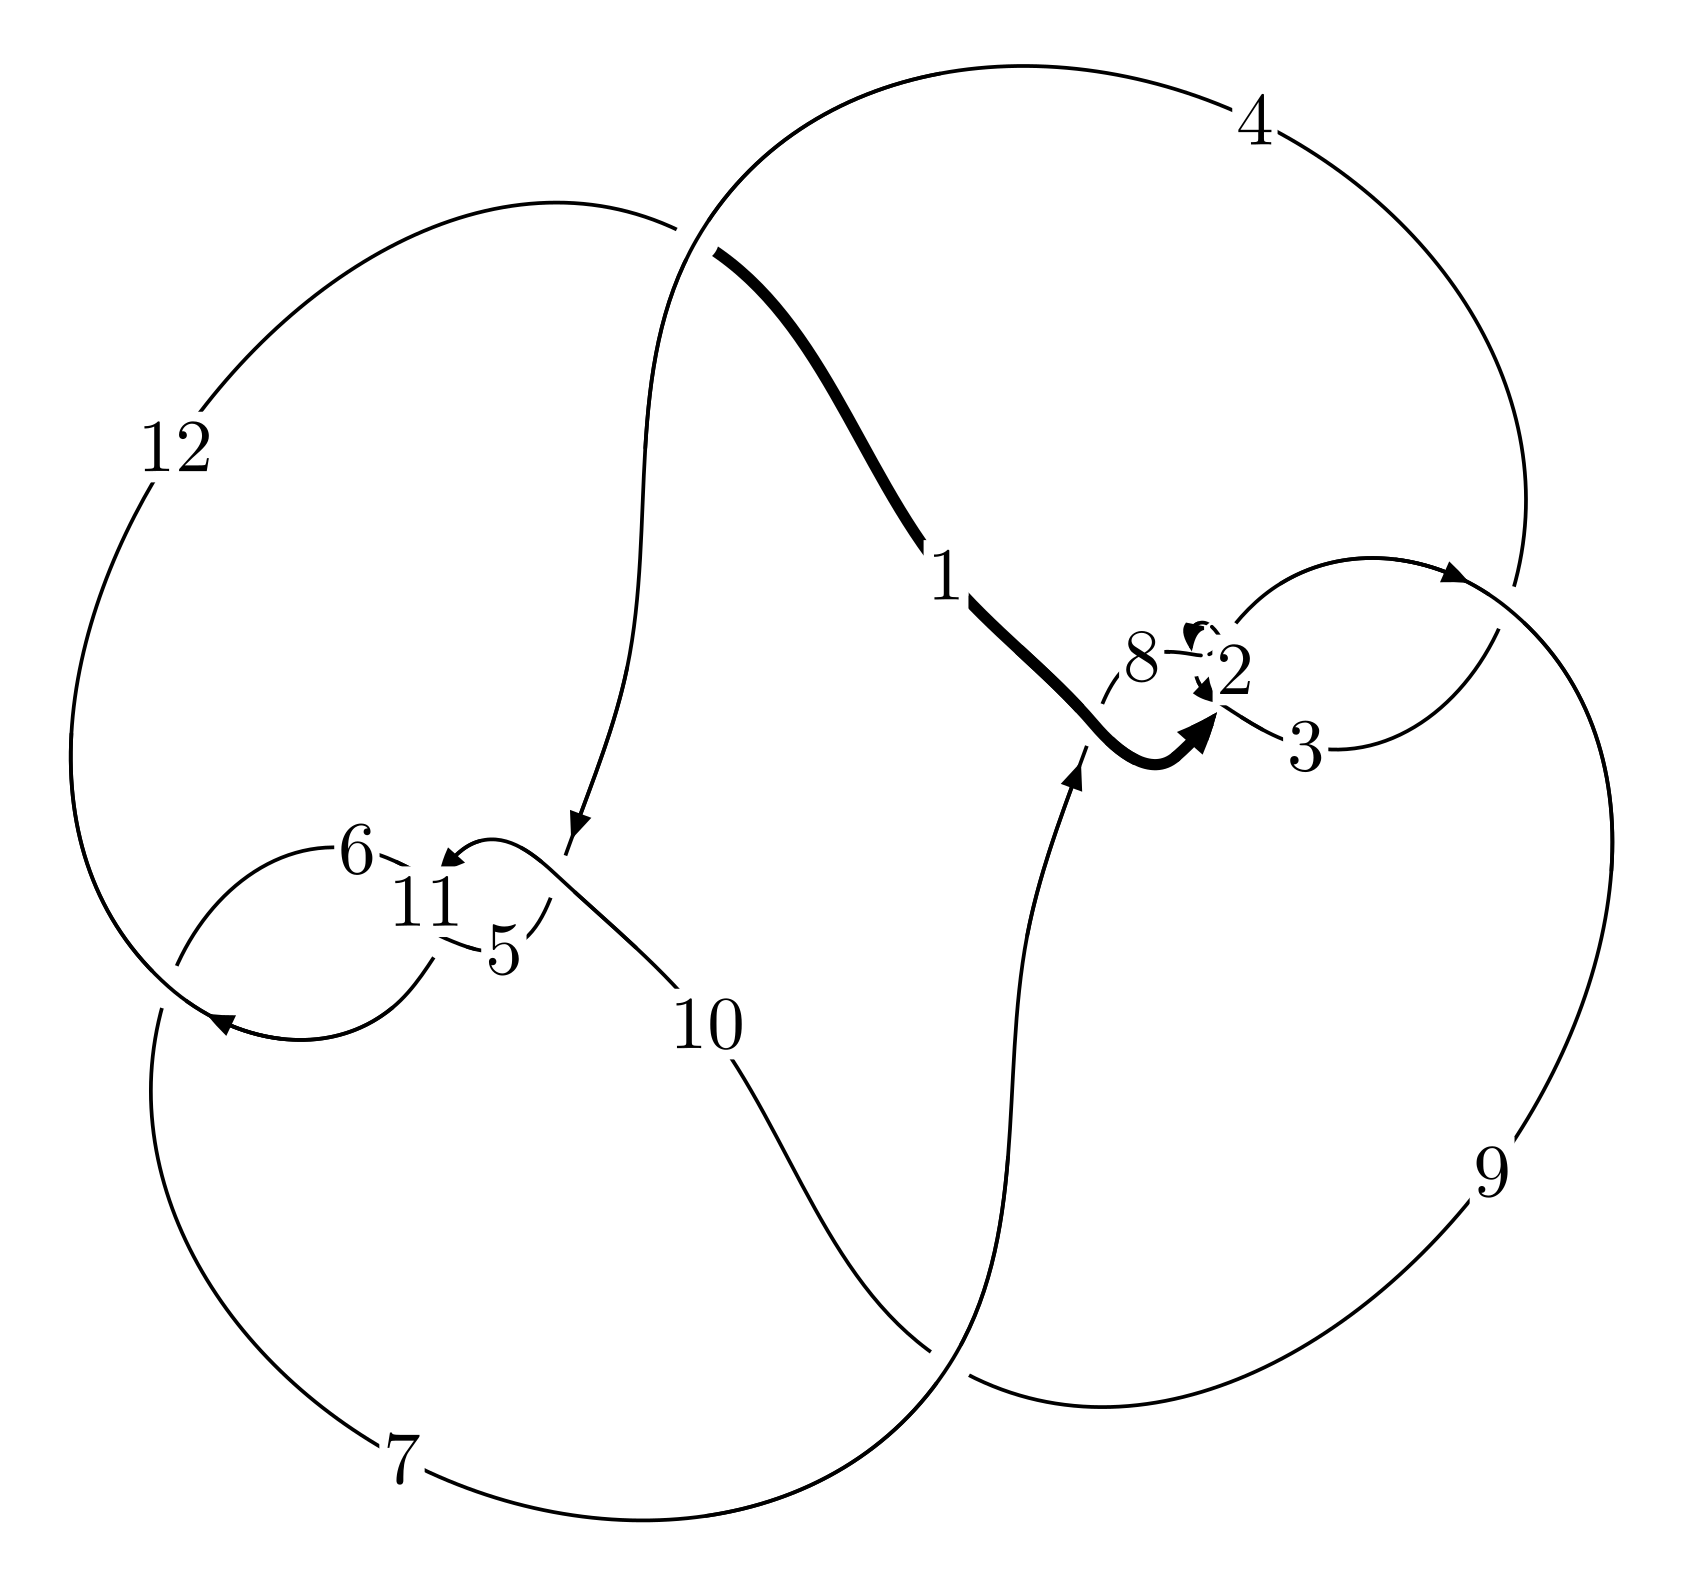
\includegraphics[width=112pt]{../../../GIT/diagram.site/Diagrams/png/1528_12a_0727.png}\\
\ \ \ A knot diagram\footnotemark}&
\allowdisplaybreaks
\textbf{Linearized knot diagam} \\
\cline{2-2}
 &
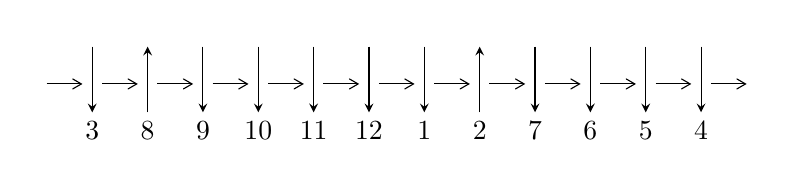
\begin{tikzpicture}[x=20pt, y=17pt]
	% nodes
	\node (C0) at (0, 0) {};
	\node (C1) at (1, 0) {};
	\node (C1U) at (1, +1) {};
	\node (C1D) at (1, -1) {3};

	\node (C2) at (2, 0) {};
	\node (C2U) at (2, +1) {};
	\node (C2D) at (2, -1) {8};

	\node (C3) at (3, 0) {};
	\node (C3U) at (3, +1) {};
	\node (C3D) at (3, -1) {9};

	\node (C4) at (4, 0) {};
	\node (C4U) at (4, +1) {};
	\node (C4D) at (4, -1) {10};

	\node (C5) at (5, 0) {};
	\node (C5U) at (5, +1) {};
	\node (C5D) at (5, -1) {11};

	\node (C6) at (6, 0) {};
	\node (C6U) at (6, +1) {};
	\node (C6D) at (6, -1) {12};

	\node (C7) at (7, 0) {};
	\node (C7U) at (7, +1) {};
	\node (C7D) at (7, -1) {1};

	\node (C8) at (8, 0) {};
	\node (C8U) at (8, +1) {};
	\node (C8D) at (8, -1) {2};

	\node (C9) at (9, 0) {};
	\node (C9U) at (9, +1) {};
	\node (C9D) at (9, -1) {7};

	\node (C10) at (10, 0) {};
	\node (C10U) at (10, +1) {};
	\node (C10D) at (10, -1) {6};

	\node (C11) at (11, 0) {};
	\node (C11U) at (11, +1) {};
	\node (C11D) at (11, -1) {5};

	\node (C12) at (12, 0) {};
	\node (C12U) at (12, +1) {};
	\node (C12D) at (12, -1) {4};
	\node (C13) at (13, 0) {};

	% arrows
	\draw[->,>={angle 60}]
	(C0) edge (C1) (C1) edge (C2) (C2) edge (C3) (C3) edge (C4) (C4) edge (C5) (C5) edge (C6) (C6) edge (C7) (C7) edge (C8) (C8) edge (C9) (C9) edge (C10) (C10) edge (C11) (C11) edge (C12) (C12) edge (C13) ;	\draw[->,>=stealth]
	(C1U) edge (C1D) (C2D) edge (C2U) (C3U) edge (C3D) (C4U) edge (C4D) (C5U) edge (C5D) (C6U) edge (C6D) (C7U) edge (C7D) (C8D) edge (C8U) (C9U) edge (C9D) (C10U) edge (C10D) (C11U) edge (C11D) (C12U) edge (C12D) ;
	\end{tikzpicture} \\
\hhline{~~} \\& 
\textbf{Solving Sequence} \\ \cline{2-2} 
 &
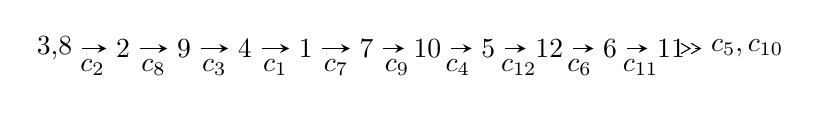
\begin{tikzpicture}[x=22pt, y=7pt]
	% node
	\node (A0) at (-1/8, 0) {3,8};
	\node (A1) at (1, 0) {2};
	\node (A2) at (2, 0) {9};
	\node (A3) at (3, 0) {4};
	\node (A4) at (4, 0) {1};
	\node (A5) at (5, 0) {7};
	\node (A6) at (6, 0) {10};
	\node (A7) at (7, 0) {5};
	\node (A8) at (8, 0) {12};
	\node (A9) at (9, 0) {6};
	\node (A10) at (10, 0) {11};
	\node (C1) at (1/2, -1) {$c_{2}$};
	\node (C2) at (3/2, -1) {$c_{8}$};
	\node (C3) at (5/2, -1) {$c_{3}$};
	\node (C4) at (7/2, -1) {$c_{1}$};
	\node (C5) at (9/2, -1) {$c_{7}$};
	\node (C6) at (11/2, -1) {$c_{9}$};
	\node (C7) at (13/2, -1) {$c_{4}$};
	\node (C8) at (15/2, -1) {$c_{12}$};
	\node (C9) at (17/2, -1) {$c_{6}$};
	\node (C10) at (19/2, -1) {$c_{11}$};
	\node (A11) at (45/4, 0) {$c_{5},c_{10}$};

	% edge
	\draw[->,>=stealth]	
	(A0) edge (A1) (A1) edge (A2) (A2) edge (A3) (A3) edge (A4) (A4) edge (A5) (A5) edge (A6) (A6) edge (A7) (A7) edge (A8) (A8) edge (A9) (A9) edge (A10) ;
	\draw[->>,>={angle 60}]	
	(A10) edge (A11);
\end{tikzpicture} \\ 

\end{tabular} \\

\footnotetext{
The image of knot diagram is generated by the software ``\textbf{Draw programme}" developed by Andrew Bartholomew(\url{http://www.layer8.co.uk/maths/draw/index.htm\#Running-draw}), where we modified some parts for our purpose(\url{https://github.com/CATsTAILs/LinksPainter}).
}\phantom \\ \newline 
\centering \textbf{Ideals for irreducible components\footnotemark of $X_{\text{par}}$} 
 
\begin{align*}
I^u_{1}&=\langle 
u^{78}- u^{77}+\cdots+u-1\rangle \\
\\
\end{align*}
\raggedright * 1 irreducible components of $\dim_{\mathbb{C}}=0$, with total 78 representations.\\
\footnotetext{All coefficients of polynomials are rational numbers. But the coefficients are sometimes approximated in decimal forms when there is not enough margin.}
\newpage
\renewcommand{\arraystretch}{1}
\centering \section*{I. $I^u_{1}= \langle u^{78}- u^{77}+\cdots+u-1 \rangle$}
\flushleft \textbf{(i) Arc colorings}\\
\begin{tabular}{m{7pt} m{180pt} m{7pt} m{180pt} }
\flushright $a_{3}=$&$\begin{pmatrix}1\\0\end{pmatrix}$ \\
\flushright $a_{8}=$&$\begin{pmatrix}0\\u\end{pmatrix}$ \\
\flushright $a_{2}=$&$\begin{pmatrix}1\\u^2\end{pmatrix}$ \\
\flushright $a_{9}=$&$\begin{pmatrix}u\\u^3+u\end{pmatrix}$ \\
\flushright $a_{4}=$&$\begin{pmatrix}u^4+u^2+1\\u^6+2 u^4+u^2\end{pmatrix}$ \\
\flushright $a_{1}=$&$\begin{pmatrix}u^2+1\\u^2\end{pmatrix}$ \\
\flushright $a_{7}=$&$\begin{pmatrix}u^5+2 u^3+u\\u^5+u^3+u\end{pmatrix}$ \\
\flushright $a_{10}=$&$\begin{pmatrix}- u^{13}-4 u^{11}-7 u^9-6 u^7-2 u^5+u\\- u^{13}-3 u^{11}-5 u^9-4 u^7-2 u^5+u^3+u\end{pmatrix}$ \\
\flushright $a_{5}=$&$\begin{pmatrix}- u^{32}-9 u^{30}+\cdots+2 u^2+1\\- u^{32}-8 u^{30}+\cdots+4 u^4+2 u^2\end{pmatrix}$ \\
\flushright $a_{12}=$&$\begin{pmatrix}- u^{12}-3 u^{10}-5 u^8-4 u^6-2 u^4+u^2+1\\- u^{14}-4 u^{12}-7 u^{10}-6 u^8-2 u^6+u^2\end{pmatrix}$ \\
\flushright $a_{6}=$&$\begin{pmatrix}- u^{31}-8 u^{29}+\cdots+4 u^3+2 u\\- u^{33}-9 u^{31}+\cdots+2 u^3+u\end{pmatrix}$ \\
\flushright $a_{11}=$&$\begin{pmatrix}- u^{77}-20 u^{75}+\cdots-2 u^3+u\\- u^{77}+u^{76}+\cdots+u-1\end{pmatrix}$\\&\end{tabular}
\flushleft \textbf{(ii) Obstruction class $= -1$}\\~\\
\flushleft \textbf{(iii) Cusp Shapes $= 4 u^{77}-4 u^{76}+\cdots+24 u^3-6$}\\~\\
\newpage\renewcommand{\arraystretch}{1}
\flushleft \textbf{(iv) u-Polynomials at the component}\newline \\
\begin{tabular}{m{50pt}|m{274pt}}
Crossings & \hspace{64pt}u-Polynomials at each crossing \\
\hline $$\begin{aligned}c_{1}\end{aligned}$$&$\begin{aligned}
&u^{78}+41 u^{77}+\cdots- u+1
\end{aligned}$\\
\hline $$\begin{aligned}c_{2},c_{8}\end{aligned}$$&$\begin{aligned}
&u^{78}- u^{77}+\cdots+u-1
\end{aligned}$\\
\hline $$\begin{aligned}c_{3},c_{7}\end{aligned}$$&$\begin{aligned}
&u^{78}+u^{77}+\cdots-377 u-53
\end{aligned}$\\
\hline $$\begin{aligned}c_{4},c_{6}\end{aligned}$$&$\begin{aligned}
&u^{78}- u^{77}+\cdots-3 u-1
\end{aligned}$\\
\hline $$\begin{aligned}c_{5},c_{10},c_{11}\end{aligned}$$&$\begin{aligned}
&u^{78}+u^{77}+\cdots-3 u-1
\end{aligned}$\\
\hline $$\begin{aligned}c_{9},c_{12}\end{aligned}$$&$\begin{aligned}
&u^{78}-7 u^{77}+\cdots+17 u+5
\end{aligned}$\\
\hline
\end{tabular}\\~\\
\newpage\renewcommand{\arraystretch}{1}
\flushleft \textbf{(v) Riley Polynomials at the component}\newline \\
\begin{tabular}{m{50pt}|m{274pt}}
Crossings & \hspace{64pt}Riley Polynomials at each crossing \\
\hline $$\begin{aligned}c_{1}\end{aligned}$$&$\begin{aligned}
&y^{78}-7 y^{77}+\cdots-25 y+1
\end{aligned}$\\
\hline $$\begin{aligned}c_{2},c_{8}\end{aligned}$$&$\begin{aligned}
&y^{78}+41 y^{77}+\cdots- y+1
\end{aligned}$\\
\hline $$\begin{aligned}c_{3},c_{7}\end{aligned}$$&$\begin{aligned}
&y^{78}-55 y^{77}+\cdots-132377 y+2809
\end{aligned}$\\
\hline $$\begin{aligned}c_{4},c_{6}\end{aligned}$$&$\begin{aligned}
&y^{78}-43 y^{77}+\cdots- y+1
\end{aligned}$\\
\hline $$\begin{aligned}c_{5},c_{10},c_{11}\end{aligned}$$&$\begin{aligned}
&y^{78}+65 y^{77}+\cdots- y+1
\end{aligned}$\\
\hline $$\begin{aligned}c_{9},c_{12}\end{aligned}$$&$\begin{aligned}
&y^{78}+45 y^{77}+\cdots+351 y+25
\end{aligned}$\\
\hline
\end{tabular}\\~\\
\newpage\flushleft \textbf{(vi) Complex Volumes and Cusp Shapes}
$$\begin{array}{c|c|c}  
\text{Solutions to }I^u_{1}& \I (\text{vol} + \sqrt{-1}CS) & \text{Cusp shape}\\
 \hline 
\begin{aligned}
u &= -0.578901 + 0.820690 I\end{aligned}
 & \phantom{-}5.58025 - 9.66694 I & -3.02999 + 8.66670 I \\ \hline\begin{aligned}
u &= -0.578901 - 0.820690 I\end{aligned}
 & \phantom{-}5.58025 + 9.66694 I & -3.02999 - 8.66670 I \\ \hline\begin{aligned}
u &= \phantom{-}0.564180 + 0.819146 I\end{aligned}
 & \phantom{-}0.77390 + 5.79656 I & -8.00000 - 7.45829 I \\ \hline\begin{aligned}
u &= \phantom{-}0.564180 - 0.819146 I\end{aligned}
 & \phantom{-}0.77390 - 5.79656 I & -8.00000 + 7.45829 I \\ \hline\begin{aligned}
u &= \phantom{-}0.126915 + 0.981484 I\end{aligned}
 & -0.758555 - 1.060210 I & -12.70969 + 0. I\phantom{ +0.000000I} \\ \hline\begin{aligned}
u &= \phantom{-}0.126915 - 0.981484 I\end{aligned}
 & -0.758555 + 1.060210 I & -12.70969 + 0. I\phantom{ +0.000000I} \\ \hline\begin{aligned}
u &= -0.188582 + 0.998058 I\end{aligned}
 & -4.15960 - 2.63280 I & -15.9415 + 4.4696 I \\ \hline\begin{aligned}
u &= -0.188582 - 0.998058 I\end{aligned}
 & -4.15960 + 2.63280 I & -15.9415 - 4.4696 I \\ \hline\begin{aligned}
u &= \phantom{-}0.586068 + 0.770581 I\end{aligned}
 & \phantom{-}9.87181 + 2.31305 I & \phantom{-}0.87298 - 3.50878 I \\ \hline\begin{aligned}
u &= \phantom{-}0.586068 - 0.770581 I\end{aligned}
 & \phantom{-}9.87181 - 2.31305 I & \phantom{-}0.87298 + 3.50878 I \\ \hline\begin{aligned}
u &= -0.524243 + 0.802290 I\end{aligned}
 & \phantom{-}3.35909 - 2.09213 I & -4.14215 + 3.78128 I \\ \hline\begin{aligned}
u &= -0.524243 - 0.802290 I\end{aligned}
 & \phantom{-}3.35909 + 2.09213 I & -4.14215 - 3.78128 I \\ \hline\begin{aligned}
u &= \phantom{-}0.228006 + 1.032790 I\end{aligned}
 & \phantom{-}0.23030 + 6.39957 I & \phantom{-0.000000 } 0 \\ \hline\begin{aligned}
u &= \phantom{-}0.228006 - 1.032790 I\end{aligned}
 & \phantom{-}0.23030 - 6.39957 I & \phantom{-0.000000 } 0 \\ \hline\begin{aligned}
u &= -0.536678 + 0.763397 I\end{aligned}
 & \phantom{-}3.42631 - 2.16410 I & -2.80015 + 4.33324 I \\ \hline\begin{aligned}
u &= -0.536678 - 0.763397 I\end{aligned}
 & \phantom{-}3.42631 + 2.16410 I & -2.80015 - 4.33324 I \\ \hline\begin{aligned}
u &= -0.587628 + 0.712984 I\end{aligned}
 & \phantom{-}5.88785 + 5.05739 I & -2.00225 - 2.01742 I \\ \hline\begin{aligned}
u &= -0.587628 - 0.712984 I\end{aligned}
 & \phantom{-}5.88785 - 5.05739 I & -2.00225 + 2.01742 I \\ \hline\begin{aligned}
u &= \phantom{-}0.566932 + 0.711290 I\end{aligned}
 & \phantom{-}1.08131 - 1.28672 I & -6.69250 + 0.65759 I \\ \hline\begin{aligned}
u &= \phantom{-}0.566932 - 0.711290 I\end{aligned}
 & \phantom{-}1.08131 + 1.28672 I & -6.69250 - 0.65759 I \\ \hline\begin{aligned}
u &= \phantom{-}0.436106 + 1.077000 I\end{aligned}
 & \phantom{-}0.62586 + 6.51824 I & \phantom{-0.000000 } 0 \\ \hline\begin{aligned}
u &= \phantom{-}0.436106 - 1.077000 I\end{aligned}
 & \phantom{-}0.62586 - 6.51824 I & \phantom{-0.000000 } 0 \\ \hline\begin{aligned}
u &= \phantom{-}0.794491 + 0.182712 I\end{aligned}
 & \phantom{-}2.53319 - 10.66910 I & -4.99373 + 6.90803 I \\ \hline\begin{aligned}
u &= \phantom{-}0.794491 - 0.182712 I\end{aligned}
 & \phantom{-}2.53319 + 10.66910 I & -4.99373 - 6.90803 I \\ \hline\begin{aligned}
u &= -0.787999 + 0.174370 I\end{aligned}
 & -2.22038 + 6.64799 I & -9.69976 - 5.44355 I \\ \hline\begin{aligned}
u &= -0.787999 - 0.174370 I\end{aligned}
 & -2.22038 - 6.64799 I & -9.69976 + 5.44355 I \\ \hline\begin{aligned}
u &= -0.454756 + 0.666376 I\end{aligned}
 & \phantom{-}3.63436 - 1.97058 I & -2.14073 + 3.77447 I \\ \hline\begin{aligned}
u &= -0.454756 - 0.666376 I\end{aligned}
 & \phantom{-}3.63436 + 1.97058 I & -2.14073 - 3.77447 I \\ \hline\begin{aligned}
u &= -0.336071 + 1.154890 I\end{aligned}
 & \phantom{-}3.31959 + 0.07641 I & \phantom{-0.000000 } 0 \\ \hline\begin{aligned}
u &= -0.336071 - 1.154890 I\end{aligned}
 & \phantom{-}3.31959 - 0.07641 I & \phantom{-0.000000 } 0\\
 \hline 
 \end{array}$$\newpage$$\begin{array}{c|c|c}  
\text{Solutions to }I^u_{1}& \I (\text{vol} + \sqrt{-1}CS) & \text{Cusp shape}\\
 \hline 
\begin{aligned}
u &= -0.417832 + 1.133420 I\end{aligned}
 & -3.94716 - 3.62664 I & \phantom{-0.000000 } 0 \\ \hline\begin{aligned}
u &= -0.417832 - 1.133420 I\end{aligned}
 & -3.94716 + 3.62664 I & \phantom{-0.000000 } 0 \\ \hline\begin{aligned}
u &= \phantom{-}0.773320 + 0.160143 I\end{aligned}
 & \phantom{-}0.56432 - 2.64520 I & -6.76601 + 1.68251 I \\ \hline\begin{aligned}
u &= \phantom{-}0.773320 - 0.160143 I\end{aligned}
 & \phantom{-}0.56432 + 2.64520 I & -6.76601 - 1.68251 I \\ \hline\begin{aligned}
u &= -0.758374 + 0.212450 I\end{aligned}
 & \phantom{-}7.37800 + 3.50504 I & -0.66245 - 2.81741 I \\ \hline\begin{aligned}
u &= -0.758374 - 0.212450 I\end{aligned}
 & \phantom{-}7.37800 - 3.50504 I & -0.66245 + 2.81741 I \\ \hline\begin{aligned}
u &= \phantom{-}0.374455 + 1.156650 I\end{aligned}
 & -2.70435 + 0.70430 I & \phantom{-0.000000 } 0 \\ \hline\begin{aligned}
u &= \phantom{-}0.374455 - 1.156650 I\end{aligned}
 & -2.70435 - 0.70430 I & \phantom{-0.000000 } 0 \\ \hline\begin{aligned}
u &= -0.771864 + 0.021540 I\end{aligned}
 & -2.45068 + 4.03806 I & -9.57286 - 3.60585 I \\ \hline\begin{aligned}
u &= -0.771864 - 0.021540 I\end{aligned}
 & -2.45068 - 4.03806 I & -9.57286 + 3.60585 I \\ \hline\begin{aligned}
u &= \phantom{-}0.770221\phantom{ +0.000000I}\end{aligned}
 & -6.34762\phantom{ +0.000000I} & -13.9660\phantom{ +0.000000I} \\ \hline\begin{aligned}
u &= \phantom{-}0.512327 + 1.132430 I\end{aligned}
 & \phantom{-}1.51982 + 0.85953 I & \phantom{-0.000000 } 0 \\ \hline\begin{aligned}
u &= \phantom{-}0.512327 - 1.132430 I\end{aligned}
 & \phantom{-}1.51982 - 0.85953 I & \phantom{-0.000000 } 0 \\ \hline\begin{aligned}
u &= \phantom{-}0.369523 + 1.188730 I\end{aligned}
 & -3.41759 + 1.14172 I & \phantom{-0.000000 } 0 \\ \hline\begin{aligned}
u &= \phantom{-}0.369523 - 1.188730 I\end{aligned}
 & -3.41759 - 1.14172 I & \phantom{-0.000000 } 0 \\ \hline\begin{aligned}
u &= \phantom{-}0.733419 + 0.176644 I\end{aligned}
 & \phantom{-}1.09971 - 2.87927 I & -4.76575 + 4.38124 I \\ \hline\begin{aligned}
u &= \phantom{-}0.733419 - 0.176644 I\end{aligned}
 & \phantom{-}1.09971 + 2.87927 I & -4.76575 - 4.38124 I \\ \hline\begin{aligned}
u &= -0.356853 + 1.193820 I\end{aligned}
 & -6.31821 + 2.88878 I & \phantom{-0.000000 } 0 \\ \hline\begin{aligned}
u &= -0.356853 - 1.193820 I\end{aligned}
 & -6.31821 - 2.88878 I & \phantom{-0.000000 } 0 \\ \hline\begin{aligned}
u &= \phantom{-}0.349156 + 1.196430 I\end{aligned}
 & -1.62767 - 6.93096 I & \phantom{-0.000000 } 0 \\ \hline\begin{aligned}
u &= \phantom{-}0.349156 - 1.196430 I\end{aligned}
 & -1.62767 + 6.93096 I & \phantom{-0.000000 } 0 \\ \hline\begin{aligned}
u &= -0.498310 + 1.142680 I\end{aligned}
 & -3.33385 - 4.23839 I & \phantom{-0.000000 } 0 \\ \hline\begin{aligned}
u &= -0.498310 - 1.142680 I\end{aligned}
 & -3.33385 + 4.23839 I & \phantom{-0.000000 } 0 \\ \hline\begin{aligned}
u &= \phantom{-}0.153987 + 0.736438 I\end{aligned}
 & -0.528165 + 0.894862 I & -9.40631 - 7.34603 I \\ \hline\begin{aligned}
u &= \phantom{-}0.153987 - 0.736438 I\end{aligned}
 & -0.528165 - 0.894862 I & -9.40631 + 7.34603 I \\ \hline\begin{aligned}
u &= \phantom{-}0.694959 + 0.256300 I\end{aligned}
 & \phantom{-}4.06421 + 3.75062 I & -2.75383 - 2.73497 I \\ \hline\begin{aligned}
u &= \phantom{-}0.694959 - 0.256300 I\end{aligned}
 & \phantom{-}4.06421 - 3.75062 I & -2.75383 + 2.73497 I \\ \hline\begin{aligned}
u &= \phantom{-}0.508450 + 1.163050 I\end{aligned}
 & -1.75841 + 7.54329 I & \phantom{-0.000000 } 0 \\ \hline\begin{aligned}
u &= \phantom{-}0.508450 - 1.163050 I\end{aligned}
 & -1.75841 - 7.54329 I & \phantom{-0.000000 } 0 \\ \hline\begin{aligned}
u &= -0.524201 + 1.160870 I\end{aligned}
 & \phantom{-}4.60438 - 8.30483 I & \phantom{-0.000000 } 0\\
 \hline 
 \end{array}$$\newpage$$\begin{array}{c|c|c}  
\text{Solutions to }I^u_{1}& \I (\text{vol} + \sqrt{-1}CS) & \text{Cusp shape}\\
 \hline 
\begin{aligned}
u &= -0.524201 - 1.160870 I\end{aligned}
 & \phantom{-}4.60438 + 8.30483 I & \phantom{-0.000000 } 0 \\ \hline\begin{aligned}
u &= -0.440440 + 1.197610 I\end{aligned}
 & -6.00210 - 0.27240 I & \phantom{-0.000000 } 0 \\ \hline\begin{aligned}
u &= -0.440440 - 1.197610 I\end{aligned}
 & -6.00210 + 0.27240 I & \phantom{-0.000000 } 0 \\ \hline\begin{aligned}
u &= \phantom{-}0.449901 + 1.196690 I\end{aligned}
 & -9.82963 + 4.37268 I & \phantom{-0.000000 } 0 \\ \hline\begin{aligned}
u &= \phantom{-}0.449901 - 1.196690 I\end{aligned}
 & -9.82963 - 4.37268 I & \phantom{-0.000000 } 0 \\ \hline\begin{aligned}
u &= -0.458822 + 1.196290 I\end{aligned}
 & -5.87231 - 8.47661 I & \phantom{-0.000000 } 0 \\ \hline\begin{aligned}
u &= -0.458822 - 1.196290 I\end{aligned}
 & -5.87231 + 8.47661 I & \phantom{-0.000000 } 0 \\ \hline\begin{aligned}
u &= \phantom{-}0.513114 + 1.178070 I\end{aligned}
 & -2.41053 + 7.41642 I & \phantom{-0.000000 } 0 \\ \hline\begin{aligned}
u &= \phantom{-}0.513114 - 1.178070 I\end{aligned}
 & -2.41053 - 7.41642 I & \phantom{-0.000000 } 0 \\ \hline\begin{aligned}
u &= -0.520654 + 1.179930 I\end{aligned}
 & -5.17476 - 11.49350 I & \phantom{-0.000000 } 0 \\ \hline\begin{aligned}
u &= -0.520654 - 1.179930 I\end{aligned}
 & -5.17476 + 11.49350 I & \phantom{-0.000000 } 0 \\ \hline\begin{aligned}
u &= \phantom{-}0.524977 + 1.180090 I\end{aligned}
 & -0.4034 + 15.5519 I & \phantom{-0.000000 } 0 \\ \hline\begin{aligned}
u &= \phantom{-}0.524977 - 1.180090 I\end{aligned}
 & -0.4034 - 15.5519 I & \phantom{-0.000000 } 0 \\ \hline\begin{aligned}
u &= -0.663438 + 0.222302 I\end{aligned}
 & -0.669046 - 0.243771 I & -7.95579 + 1.30313 I \\ \hline\begin{aligned}
u &= -0.663438 - 0.222302 I\end{aligned}
 & -0.669046 + 0.243771 I & -7.95579 - 1.30313 I \\ \hline\begin{aligned}
u &= \phantom{-}0.523024 + 0.313762 I\end{aligned}
 & \phantom{-}2.74897 - 2.61573 I & -2.67127 + 3.03594 I \\ \hline\begin{aligned}
u &= \phantom{-}0.523024 - 0.313762 I\end{aligned}
 & \phantom{-}2.74897 + 2.61573 I & -2.67127 - 3.03594 I \\ \hline\begin{aligned}
u &= -0.525544\phantom{ +0.000000I}\end{aligned}
 & -0.955751\phantom{ +0.000000I} & -10.6020\phantom{ +0.000000I}\\
 \hline 
 \end{array}$$\newpage
\newpage\renewcommand{\arraystretch}{1}
\centering \section*{ II. u-Polynomials}
\begin{tabular}{m{50pt}|m{274pt}}
Crossings & \hspace{64pt}u-Polynomials at each crossing \\
\hline $$\begin{aligned}c_{1}\end{aligned}$$&$\begin{aligned}
&u^{78}+41 u^{77}+\cdots- u+1
\end{aligned}$\\
\hline $$\begin{aligned}c_{2},c_{8}\end{aligned}$$&$\begin{aligned}
&u^{78}- u^{77}+\cdots+u-1
\end{aligned}$\\
\hline $$\begin{aligned}c_{3},c_{7}\end{aligned}$$&$\begin{aligned}
&u^{78}+u^{77}+\cdots-377 u-53
\end{aligned}$\\
\hline $$\begin{aligned}c_{4},c_{6}\end{aligned}$$&$\begin{aligned}
&u^{78}- u^{77}+\cdots-3 u-1
\end{aligned}$\\
\hline $$\begin{aligned}c_{5},c_{10},c_{11}\end{aligned}$$&$\begin{aligned}
&u^{78}+u^{77}+\cdots-3 u-1
\end{aligned}$\\
\hline $$\begin{aligned}c_{9},c_{12}\end{aligned}$$&$\begin{aligned}
&u^{78}-7 u^{77}+\cdots+17 u+5
\end{aligned}$\\
\hline
\end{tabular}\newpage\renewcommand{\arraystretch}{1}
\centering \section*{ III. Riley Polynomials}
\begin{tabular}{m{50pt}|m{274pt}}
Crossings & \hspace{64pt}Riley Polynomials at each crossing \\
\hline $$\begin{aligned}c_{1}\end{aligned}$$&$\begin{aligned}
&y^{78}-7 y^{77}+\cdots-25 y+1
\end{aligned}$\\
\hline $$\begin{aligned}c_{2},c_{8}\end{aligned}$$&$\begin{aligned}
&y^{78}+41 y^{77}+\cdots- y+1
\end{aligned}$\\
\hline $$\begin{aligned}c_{3},c_{7}\end{aligned}$$&$\begin{aligned}
&y^{78}-55 y^{77}+\cdots-132377 y+2809
\end{aligned}$\\
\hline $$\begin{aligned}c_{4},c_{6}\end{aligned}$$&$\begin{aligned}
&y^{78}-43 y^{77}+\cdots- y+1
\end{aligned}$\\
\hline $$\begin{aligned}c_{5},c_{10},c_{11}\end{aligned}$$&$\begin{aligned}
&y^{78}+65 y^{77}+\cdots- y+1
\end{aligned}$\\
\hline $$\begin{aligned}c_{9},c_{12}\end{aligned}$$&$\begin{aligned}
&y^{78}+45 y^{77}+\cdots+351 y+25
\end{aligned}$\\
\hline
\end{tabular}
\vskip 2pc
\end{document}